%!TEX root = ../main.tex

\section{Results}
\label{sec:Results}

We analyse the convergence of the numerical scheme to a known analytical solution 
\begin{equation}
\label{eq:analytical-sol-known}
\phi(x,y,z)=\frac{-1}{4\pi\sqrt{(x-1)^2+(y-0.5)^2+(z-0.5)^2}} 
\end{equation}

for a mixed Dirichlet-Neumann problem on the domain configurations illustrated in Fig.~\ref{fig:original-2} and Fig.~\ref{fig:original-6}.

The first test case considers a sphere of radius $R=1$ and centered in $O=(0,0,0)$. On the left of Fig.~\ref{fig:original-2} we show the initial grid, represented by a simple cube. Dirichlet boundary conditions are applied to the red faces, while Neumann boundary conditions are applied to the blue faces. The right image represents the mesh obtained after 3 global refinement cycles. The possibility to introduce a very coarse initial discretisation of the domain is a key feature of the $\pi$\texttt{-BEM} library.

\begin{figure}[htp]
\begin{center}
    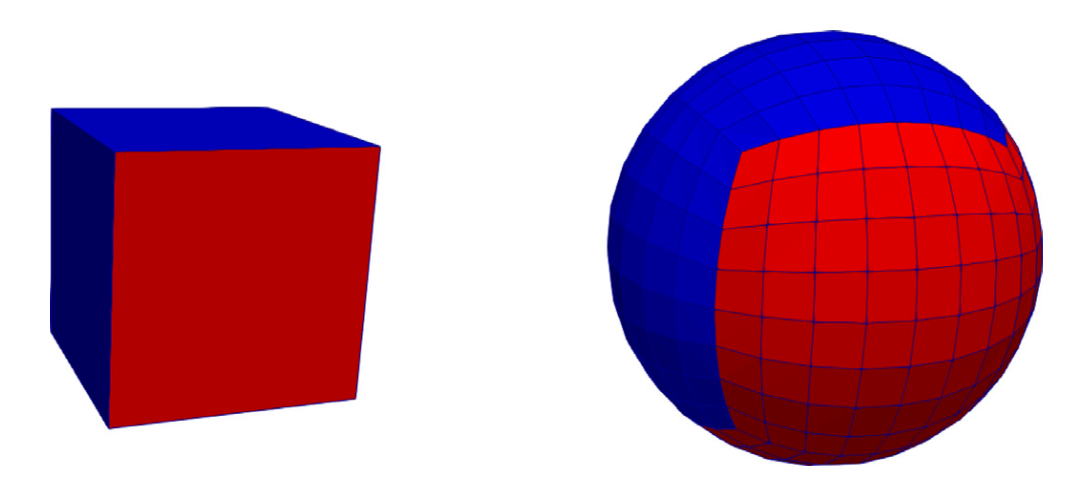
\includegraphics[width=8.4cm]{original-2}    % The printed column width is 8.4 cm.
    \caption{Mesh configuration for the sphere test case with mixed boundary conditions.} 
    \label{fig:original-2}
\end{center}
\end{figure}

While Fig.~\ref{fig:original-3} shows the computed solution $\phi$ over $98304$ cells, Fig.~\ref{fig:original-4} presents the convergence analysis for both the potential (on the left) and its normal derivative (on the right). We obtained a first order convergence on $\phi$ using $Q_1$ elements for both $L_2$ and $L_\infty$ norm. 

\begin{figure}[htp]
\begin{center}
    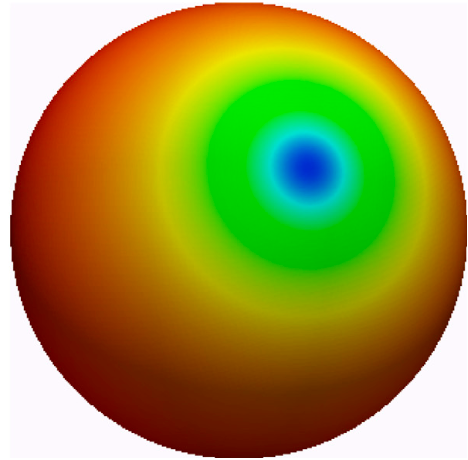
\includegraphics[width=4.2cm]{original-3}    % The printed column width is 8.4 cm.
    \caption{Sphere test case. The colours represent the magnitude of the exact solution $\phi$.} 
    \label{fig:original-3}
\end{center}
\end{figure}

\begin{figure*}[htp]
\begin{center}
    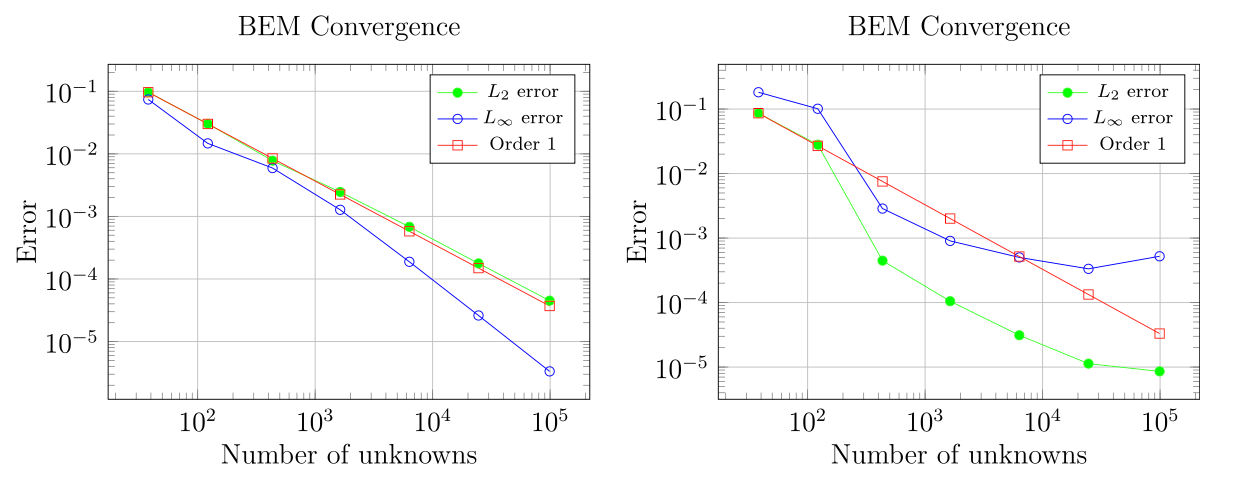
\includegraphics[width=14cm]{original-4}    % The printed column width is 8.4 cm.
    \caption{Convergence analysis for the error in a mixed Dirichlet-Neumann problem using $Q_1$ boundary elements and the spherical mesh. On the left we plot the analysis for the variable $\phi$, on the right we depict the errors for $\frac{\partial\phi}{\partial n}$.} 
    \label{fig:original-4}
\end{center}
\end{figure*}

\newpage

For the normal derivative, we observe a more irregular behavior: initial superconvergence (greater than linear) followed by a significant decrease during the final refinement step. A closer look at the error distribution (see Fig.~\ref{fig:original-5}) suggests that the progressive refinement of an initially cubic mesh over a sphere results in the presence of few stretched cells located at the original mesh vertices. To make things worse such nodes are located at the interface between different boundary condition regions. This situation is not improved throughout the refinements of the grid, as the angle of such stretched cells remain constant for each mesh, which results in a constant error.

\begin{figure}[htp]
\begin{center}
    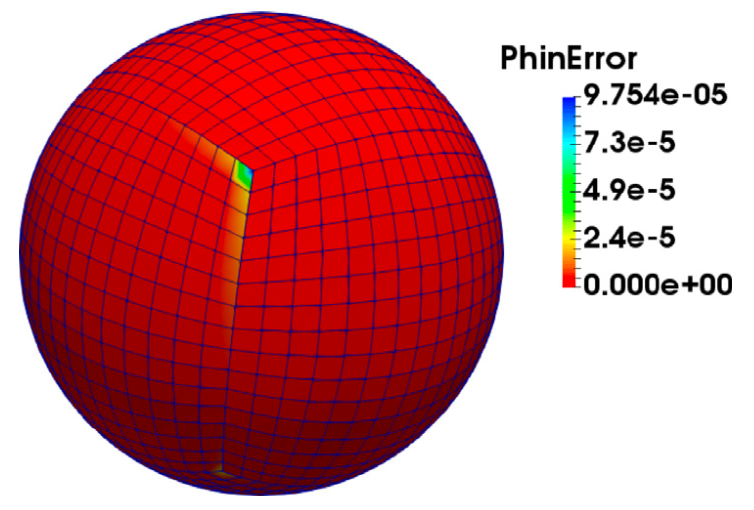
\includegraphics[width=5cm]{original-5}    % The printed column width is 8.4 cm.
    \caption{Error analysis for the potential normal derivative in the sphere test case.} 
    \label{fig:original-5}
\end{center}
\end{figure}

The second test case takes into account the truncated pyramid illustrated in Fig.~\ref{fig:original-6}.

\begin{figure}[htp]
\begin{center}
    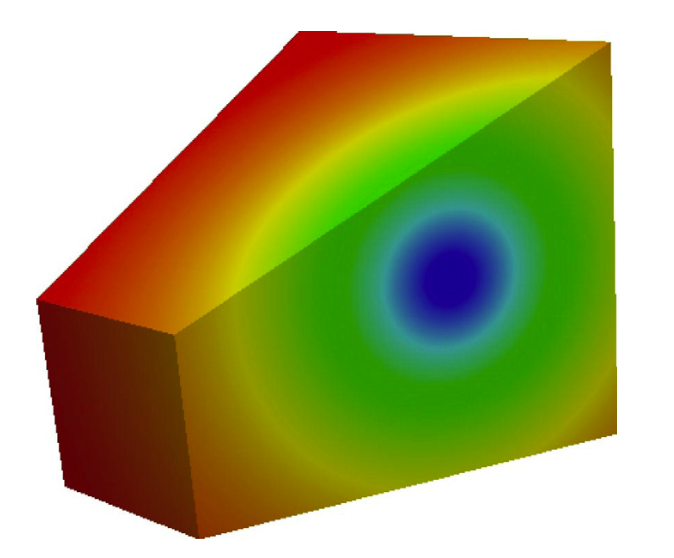
\includegraphics[width=4.2cm]{original-6}    % The printed column width is 8.4 cm.
    \caption{Truncated pyramid geometry. The colours represent the magnitude of the exact solution $\phi$.} 
    \label{fig:original-6}
\end{center}
\end{figure}

The carried out convergence analysis is shown in Fig.~\ref{fig:original-7}. Even if the domain in not the simple sphere, we obtained a first order error for $\phi$. In the case of the potential normal derivative we observe the occurrence of an error plateaux for the $L_\infty$
norm in corresponding to the last refinement level considered. A possible cause can be assessed through an inspection of the local $\frac{\partial\phi}{\partial n}$ error distribution presented in Fig.~\ref{fig:original-8}. As can be seen, the maximum error occurs in correspondence with the edge characterised by the sharpest angle of the figure.

\begin{figure*}
\begin{center}
    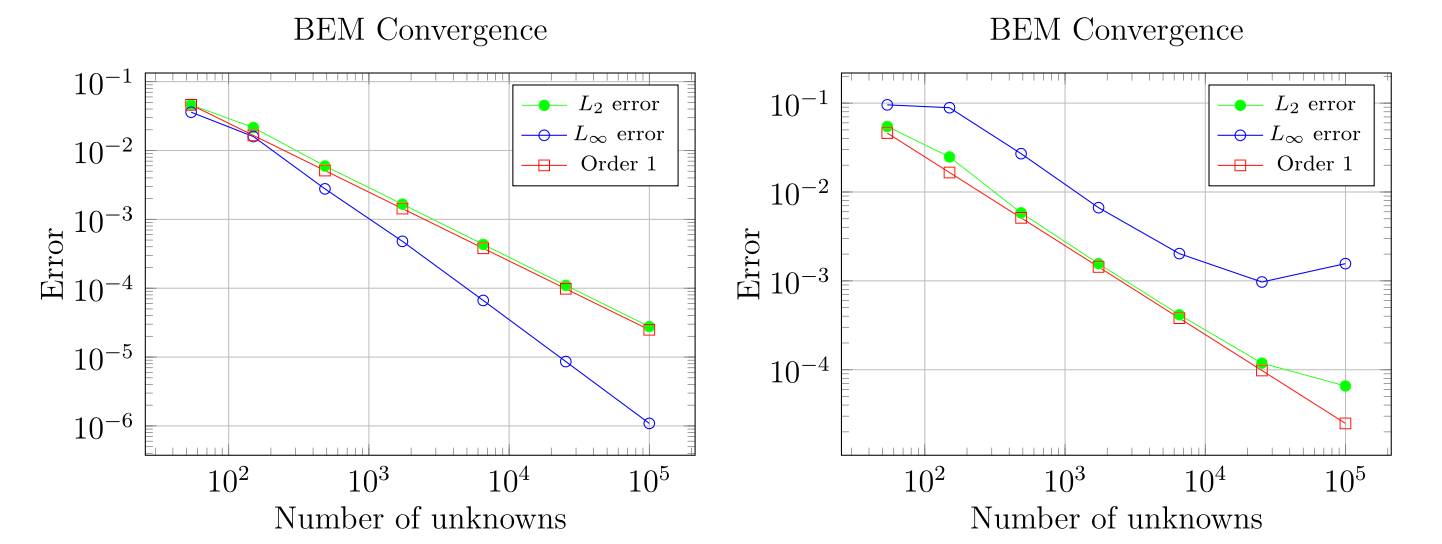
\includegraphics[width=14cm]{original-7}    % The printed column width is 8.4 cm.
    \caption{Convergence analysis for the error in a mixed Dirichlet-Neumann problem using $Q_1$ boundary elements and the truncated pyramid mesh. On the left we plot the analysis for the variable $\phi$, on the right we depict the errors for $\frac{\partial\phi}{\partial n}$.} 
    \label{fig:original-7}
\end{center}
\end{figure*}

\begin{figure}
\begin{center}
    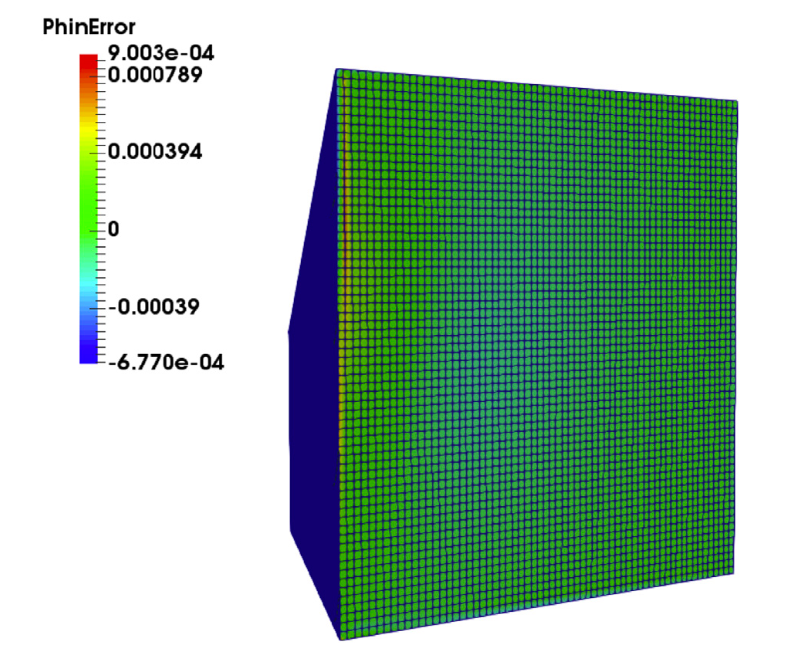
\includegraphics[width=6cm]{original-8}    % The printed column width is 8.4 cm.
    \caption{Error analysis for the potential normal derivative in the truncated pyramid test case.} 
    \label{fig:original-8}
\end{center}
\end{figure}

















